\section{Results}
\label{sec:results}

The principal results use the ten test seeds, test record pools and internally frozen code and configuration. The sections follow the original research questions: adaptation and batch labels (RQ1), domain-rule coverage and category admission (RQ2), and selective execution (RQ3), followed by ablation, transfer and sensitivity. Differences are adaptive or proposed minus comparator. Intervals are 95\% paired cluster-bootstrap intervals unless otherwise stated; differences between percentages are reported in percentage points (pp).

\subsection{H1a: Adaptive Thresholds under Drift}
\label{sec:res:h1a}

Table~\ref{tab:h1a} gives the verdict for every dataset and scenario against the primary comparator, fixed thresholds on the pooled warm-up. Table~\ref{tab:h1a:methods} lists all threshold methods under gradual drift, and Figure~\ref{fig:fpr} shows the false-positive rate batch by batch as drift grows.

\begin{table}[t]
\caption{H1a verdicts: adaptive thresholds against fixed thresholds on the pooled warm-up. FPR and recall are given as adaptive / fixed; differences are adaptive minus fixed in pp with 95\% cluster bootstrap intervals. H1a requires the FPR interval to lie below 0 and the recall interval to lie above $-1$ pp. Z has no erroneous records, so only the FPR part applies.}
\label{tab:h1a}
\footnotesize
\begin{tabular}{@{}llrrrrc@{}}
\toprule
Data & Sc. & FPR (\%) & FPR difference (pp) & Recall & Recall difference (pp) & H1a \\
\midrule
\inputtable{tables/h1a.tex}
\bottomrule
\end{tabular}
\end{table}

On the flight data, adaptive thresholds kept FPR between 4.3\% and 4.6\% as drift increased from 2\% to 30\%, whereas pooled fixed thresholds rose from 4.6\% to 7.6\% (Figure~\ref{fig:fpr}). Under gradual drift, adaptation reduced FPR by $1.55$ pp, difference $-1.55$ $[-1.59,-1.51]$, with recall 1.00 for both methods. H1a was supported in six of nine scenarios. The three failures help delimit this benefit. With mild errors and no drift (E1), the small FPR difference, $-0.03$ pp, was not distinguishable from zero. Under persistent contamination (F1/F2), adaptive recall was approximately 0.421 and fell 17.32 and 29.06 pp below the fixed comparator. Repeatedly multiplying 5\% of taxi-out values by three changed the statistics used to construct the adaptive range, allowing more corrupted values to pass. The drift gate does not prevent these profiles from entering adaptation history. Finally, the approximately 4.4\% FPR even without drift reflects legitimate long-tailed delays and taxi times; the corresponding precision was only 0.19 in scenario A. Reducing drift-induced false positives therefore does not eliminate the broader difficulty of using moment-based ranges on heavy-tailed data.

On Chicago, H1a was supported in all nine scenarios, but the FPR difference was only about $-0.03$ pp. Numerical coordinates use fixed physical bounds, and injected legitimate drift affects risk and result categories. The decomposition variant combining fixed numerical bounds with recurrence categories exactly reproduced the adaptive results. The gain is therefore attributable to category handling, which stopped repeatedly rejecting rare valid facility types absent from warm-up, rather than to numerical adaptation. Longitude contamination that remained inside the city bounding box was not detected by these rules; overall recall in F1/F2 was about 0.255. A relative non-inferiority verdict in this setting should not be mistaken for adequate absolute detection.

On Retail, H1a was not supported in any scenario. Under gradual drift, adaptive FPR was 0.80\% versus 0.75\% for fixed thresholds, difference $+0.05$ pp $[-0.10,+0.21]$, although recall was higher by approximately 2.7 pp $[+0.01,+6.0]$. H1a requires lower FPR as well as non-inferior recall, so the recall gain does not reverse the verdict. The pooled fixed range was already broad relative to the injected change: its FPR moved only from 0.68\% to 0.82\% across the drift schedule. Discrete, highly skewed quantities and prices thus offered little drift-induced false alarming for adaptation to remove. Calibrated robust rolling rules and EWMA reached lower FPR, 0.61--0.65\%, at lower recall, 0.947--0.952, illustrating a different detection trade-off rather than a uniformly best threshold policy.

\begin{figure}[t]
\centering
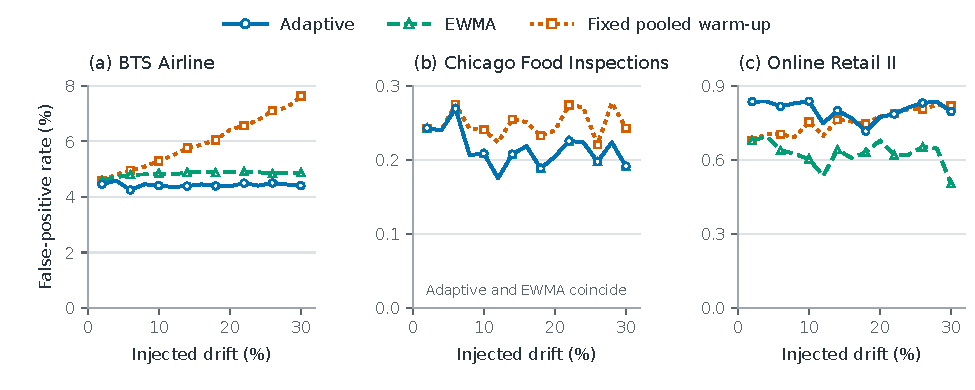
\includegraphics[width=\linewidth]{figures/h1a_fpr_over_time.pdf}
\caption{False-positive rate under gradual legitimate drift (scenario B). Each point pools false-positive and valid-record counts over ten test seeds at an evaluated batch; injected drift increases from 2\% at $B_6$ to 30\% at $B_{20}$. The panels use different vertical scales. Adaptive and EWMA results coincide on Chicago. Numerical coordinate bounds remain fixed in that dataset; its policy difference comes from category handling.}
\Description{Three line charts compare adaptive, EWMA and fixed pooled-warm-up rules. Fixed-rule false positives increase markedly under flight-data drift, while adaptive and EWMA rules remain lower. Chicago rates are much smaller and the adaptive and EWMA lines coincide. On retail data fixed and adaptive rates remain close, with EWMA lower. All panels begin at zero but have dataset-specific vertical scales.}
\label{fig:fpr}
\end{figure}

\begin{table}[t]
\caption{False-positive rate (\%) and recall of every threshold method under gradual drift (scenario B). Deequ ``default rules'' suggests constraints on the warm-up as observed; ``best case'' uses a warm-up without erroneous records and extended rules. ``Failed constraints'' counts records that violate a constraint that failed on the batch; ``any violation'' counts records that violate any suggested constraint.}
\label{tab:h1a:methods}
\footnotesize
\begin{tabular}{@{}lrrrrrr@{}}
\toprule
& \multicolumn{2}{c}{BTS} & \multicolumn{2}{c}{Chicago} & \multicolumn{2}{c}{Retail} \\
\cmidrule(lr){2-3}\cmidrule(lr){4-5}\cmidrule(l){6-7}
Method & FPR & Recall & FPR & Recall & FPR & Recall \\
\midrule
\inputtable{tables/h1a_methods.tex}
\bottomrule
\end{tabular}
\end{table}

Table~\ref{tab:h1a:methods} also shows why calibration and comparator configuration matter. Textbook robust multipliers flagged 7.6--28\% of valid flight and retail records. After warm-up calibration, rolling robust rules and EWMA came within approximately 0.4--0.5 pp of adaptive FPR on BTS. Much of the improvement over fixed bounds is therefore also obtained by these recent-history alternatives. Deequ's default suggestions on observed warm-up were tolerance-based completeness constraints, detecting the missing-value quarter of injected errors. Its favourable extended configuration detected 53--70\% of errors, but generated constraints failed on every erroneous evaluated batch and flagged roughly a fifth of valid Chicago and Retail records. These findings concern the suggested constraint sets and attribution modes tested here, not the full range of rules a practitioner could implement in Deequ.

\subsection{H1b: Separating Drift from Degradation}
\label{sec:res:h1b}

Table~\ref{tab:h1b} reports the four-class macro-F1 of every batch labeller over 600 batches per dataset (ten seeds, four scenarios, fifteen batches).

\begin{table}[t]
\caption{Four-class batch labelling in scenarios A--D. F1 is pooled macro-F1; Drift and Degr.\ are class recalls. A circle marks a comparison whose paired interval does not establish superiority of the proposed classifier. This is not an equivalence test; paired uncertainty is calculated from per-seed macro-F1.}
\label{tab:h1b}
\footnotesize
\begin{tabular}{@{}lrrrrrrrrr@{}}
\toprule
& \multicolumn{3}{c}{BTS} & \multicolumn{3}{c}{Chicago} & \multicolumn{3}{c}{Retail} \\
\cmidrule(lr){2-4}\cmidrule(lr){5-7}\cmidrule(l){8-10}
Labeller & F1 & Drift & Degr. & F1 & Drift & Degr. & F1 & Drift & Degr. \\
\midrule
\inputtable{tables/h1b.tex}
\bottomrule
\end{tabular}
\end{table}

The proposed classifier reached pooled macro-F1 of 0.966, 0.955 and 0.947 on BTS, Chicago and Retail. On BTS, it exceeded all evaluated comparators. Its effect-floor variant was closest, with a mean per-seed difference of approximately $+0.04$; calibrated TFDV followed at $+0.15$ $[0.08,0.21]$, and gated EWMA at $+0.23$ $[0.19,0.27]$. The gated fixed classifier recognised degradation but had drift-class recall of only 0.09: its fixed ranges converted valid distribution movement into higher failure rates, labelling 89\% of pure-drift batches as degraded. Adaptive thresholds lowered this share to 2.5\%, linking the batch-label improvement to their reduction of drift-induced record failures.

The same attribution does not hold on the other datasets. Chicago's gated fixed, EWMA and adaptive variants produced identical results. On Retail, gated fixed thresholds had a higher point score, 0.956 versus 0.947; the mean per-seed difference was $-0.009$ $[-0.027,+0.003]$. This establishes no detected adaptive advantage, rather than equality of the methods. Removing the gate, however, lowered pooled macro-F1 to 0.658, 0.668 and 0.720 across the three datasets. Without filtering, erroneous records changed the drift score and caused degradation-only batches to be labelled drift with degradation. The consistent contributor is therefore the gated drift evidence, with threshold adaptation adding a dataset-dependent benefit.

The documented Deequ and TFDV configurations scored below the proposed classifier on this four-state task. TFDV against the previous batch assigned almost all batches the same label; cumulative-history Deequ detected few anomalies, giving macro-F1 of approximately 0.10--0.23. Warm-up calibration raised TFDV to 0.82--0.90 and Deequ to 0.36--0.61. The AVH-inspired baseline scored about 0.28 when updated from all history and 0.43--0.56 when updated only from alarm-free batches. Its restricted metric library and the difference between anomalous-partition detection and persistent-state classification limit direct comparison with published AVH. The proposed classifier identified degradation in its onset batch in every evaluated run, and mean drift delay was 0.3, 0.9 and 0.0 batches. These controlled detection delays should not be read as guarantees for unlabelled operational incidents.

Adding a minimum drift-effect size excluded small injected shifts and lowered macro-F1 to 0.71--0.93 under labels that count every positive injected drift as drift. That reduction reflects the distinction between detecting any constructed change and prioritising operationally meaningful changes. The temporal replay examines the same trade-off without changing the primary controlled labels (Section~\ref{sec:res:replay}).

\subsection{H2a: Coverage of Validated LLM Rules}
\label{sec:res:h2a}

Table~\ref{tab:h2a} reports the recall of domain-impossible values (semantic recall) and the FPR of each rule configuration under drift (scenario S2); scenario S1 gave the same picture.

\begin{table}[t]
\caption{Semantic recall and FPR (\%) in scenario S2. Model results average five generations and ten seeds. Admitted rules pass historical screening; dictionary-only rules are authored by a third model, not human experts. Near-perfect semantic recall belongs to fixed statistical rules combined with LLM rules.}
\label{tab:h2a}
\footnotesize
\begin{tabular}{@{}lrrrrrr@{}}
\toprule
& \multicolumn{2}{c}{BTS} & \multicolumn{2}{c}{Chicago} & \multicolumn{2}{c}{Retail} \\
\cmidrule(lr){2-3}\cmidrule(lr){4-5}\cmidrule(l){6-7}
Rules & Sem.\ recall & FPR & Sem.\ recall & FPR & Sem.\ recall & FPR \\
\midrule
\inputtable{tables/h2a.tex}
\bottomrule
\end{tabular}
\end{table}

The two rule sources cover different error families. Fixed statistical rules detected invalid codes absent from warm-up, but only 3--6\% of impossible numerical flight values and less than 1\% of non-positive quantities or negative prices in Retail. Admitted LLM rules supplied restrictions such as non-negative taxi time and price, detecting the impossible numbers but missing many well-formed invalid codes in open domains. Fixed statistical rules combined with admitted LLM rules reached semantic recall of 0.996--1.00 on every dataset with either model. The gain over fixed statistical rules was $+0.48$ $[0.47,0.48]$ on BTS and $+0.49$ $[0.49,0.50]$ on Retail. Chicago was already at 1.00 because its injected semantic violations were categorical. The primary-model FPR increase was at most 0.01 pp, within the 0.5 pp tolerance. H2a is thus supported on BTS and Retail; Chicago's ceiling prevents an incremental-coverage conclusion.

Adaptive statistical rules detected only 0.07--0.13 of the same domain-impossible subset. Invalid codes recurred at 1\% in every batch and entered the allowed set after two batches. Adding LLM rules restored impossible-number detection, but not the open-domain codes; adaptive+LLM semantic recall remained 0.62--0.75. The near-perfect fixed+LLM result and the weaker adaptive+LLM result must therefore remain distinct. The separate guard experiment in Section~\ref{sec:res:h2b} investigates the category mechanism, but does not supply an integrated-system result for this configuration.

\paragraph{Admission.} Every naturally generated LLM candidate passed admission in the test runs: no candidate was malformed, exceeded the historical flag-rate ceiling or was logically implied by a kept rule. No admitted candidate exceeded 0.5\% FPR on valid evaluation records. This establishes historical and held-out compatibility for the observed candidates, not the frequency with which admission would remove harmful proposals in general. The filter acted on the dictionary-only model-authored comparison rules. Before admission they flagged 10.8\% of valid BTS records, 22.1\% of Chicago records and 0.9\% of Retail records under drift. Faulty patterns rejected carriers B6 and 9E, apostrophes in facility types and stock code POST; a category list omitted three valid inspection results. After admission their FPR was 0.00--0.03\%. Under the study's held-out-FPR criterion, no harmful comparison rule was retained and no compatible one rejected. This operational criterion is narrower than semantic correctness.

A controlled stress test supplied cases absent from the natural candidate sets: malformed, too-strict, wrong, subtly too-strict, sound, vacuous and redundant rules. All malformed rules were rejected, sound rules accepted, and vacuous or redundant rules dropped. Wrong rules initially flagging almost every valid record were rejected, dropped or relaxed; surviving rules produced 0.3--2.1 false positives per 10,000 valid records. Too-strict rules fell from 2,770--5,351 false positives per 10,000 to 1.0--3.8. This isolates the admission mechanism's filtering effect. It does not imply that relaxation preserves every useful domain distinction or estimate the natural rate of LLM rule errors.

\paragraph{Stability and cost.} Generations showed high value-level agreement on sampled and synthetic probes: 98.5--99.4\% within a model and 98.4--99.0\% between models. The primary model proposed 10.6--15.4 rules per generation and the secondary 7.8--18.0. Agreement describes the probe set, not comprehensive logical equivalence of rule suites. The thirty controlled generations have estimated cost US\$2.14, using configured prices and corrected input-token estimates as described in Section~\ref{sec:design}. Costs of per-value category judgements are reported separately.

\subsection{H2b: Guarding Category Admission}
\label{sec:res:h2b}

Table~\ref{tab:h2b} reports the share of valid and invalid novel values that each policy admitted (Figure~\ref{fig:guard} shows the same data).

\begin{table}[t]
\caption{Share of novel category values admitted, valid / invalid, over ten seeds and both novelty scenarios. Ideal: valid 1, invalid 0. Distinct values: BTS 6 valid and 6 invalid, Chicago 4 and 4, Retail 2 and 2.}
\label{tab:h2b}
\footnotesize
\begin{tabular}{@{}lrrrrrr@{}}
\toprule
& \multicolumn{2}{c}{BTS} & \multicolumn{2}{c}{Chicago} & \multicolumn{2}{c}{Retail} \\
\cmidrule(lr){2-3}\cmidrule(lr){4-5}\cmidrule(l){6-7}
Admission policy & Valid & Invalid & Valid & Invalid & Valid & Invalid \\
\midrule
\inputtable{tables/h2b.tex}
\bottomrule
\end{tabular}
\end{table}

\begin{figure}[t]
\centering
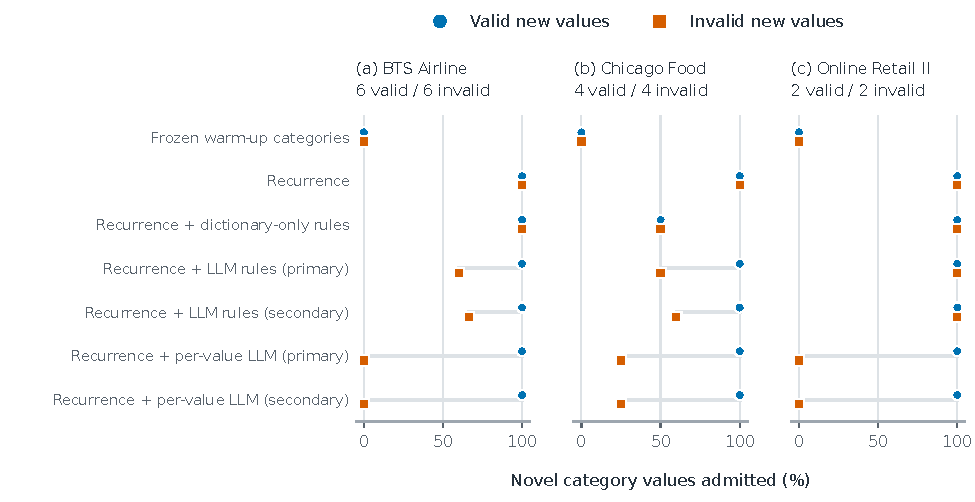
\includegraphics[width=\linewidth]{figures/h2b_category_guard.pdf}
\caption{Percentage of valid (circles) and invalid (squares) novel category values admitted by each policy, over ten test seeds and both novelty scenarios. Primary and secondary LLM policies are shown separately; the LLM-constraint rows also average the five rule generations. The ideal policy admits valid values and rejects invalid values. There are only 24 distinct values: BTS six valid and six invalid, Chicago four and four, and Retail two and two. Seed replays do not add independent semantic cases.}
\Description{Three dot-chart panels show admission percentages for seven policy/model rows. Frozen categories admit no novel values; recurrence admits all valid and invalid values. Constraint guards admit many invalid values. Per-value LLM checks admit all valid values and reject all invalid values on BTS and Retail, but admit one quarter of the invalid Chicago values. The two models have separate rows.}
\label{fig:guard}
\end{figure}

Frozen categories and unrestricted recurrence define the two extremes: the former rejects every novel value, while the latter admits every valid and invalid novel value after two batches. Constraint guards help only when their conditions separate valid membership from plausible syntax. Most open-domain LLM rules are patterns; an invalid airport code can still contain three upper-case letters. LLM-constraint guards therefore admitted 50--100\% of invalid values, recorded as unresolved where only pattern compatibility was established. Dictionary-only constraints did no better on invalid values and excluded half of Chicago's valid novelty. These outcomes distinguish syntactic admissibility from membership in a particular domain.

The per-value policy admitted all twelve valid values and rejected eleven of twelve invalid values. Both models accepted the undocumented result \emph{Not Inspected}, while rejecting \emph{Pass Conditional}, \emph{Restuarant} and \emph{Bakkery}. Their verdicts agreed on all 24 cases. H2b is supported for this per-value policy on the selected cases, but repeated seeds do not create independent semantic test sets. Values already in warm-up bypass the query, and unsure or missing verdicts revert to recurrence. Candidate verdicts were cached before replay without injected labels; the experiment does not measure live online query latency. Across development and test runs, 362 queries per model yielded token-based cost estimates of US\$2.34 and US\$3.24.

\subsection{H3: Risk-Based Check Selection}
\label{sec:res:h3}

Table~\ref{tab:h3} reports post-onset recall and the share of checks saved in the eighteen degradation and incident cases.

\begin{table}[t]
\caption{Post-onset recall and checks saved (\%, in parentheses). Bold satisfies H3 using a mean recall of at least 0.90 and positive saving. C/D recall covers all erroneous post-onset records; H1--H4 covers incident-injected records during each incident. Periodic and random schedules target the risk policy's realised standard-check execution rate; finite-run counts can differ.}
\label{tab:h3}
\footnotesize
\begin{tabular}{@{}llrrrrr@{}}
\toprule
Data & Scenario & Risk-based & Periodic & Random & Failure only & Drift only \\
\midrule
\inputtable{tables/h3.tex}
\bottomrule
\end{tabular}
\end{table}

Risk-based selection was useful in 11 of 18 cases, against 4 for cost-matched periodic and 5 for cost-matched random selection. It met the target in every sustained degradation (C, D) and in the sparse-category incident, where the risk of the affected column rose and its checks returned. It failed on sparse duplicates (post-onset recall 0.60 to 0.62), on the short two-batch incident (0.69 to 0.74) and, on the retail data, on the incident with recovery (0.87). In these cases the failure signal of a skipped check could be up to four batches old, and a sparse or short incident gives the risk score little evidence before it ends. A risk score using only the drift component was useful in 13 cases, but it saved at most 3.8\% of checks and almost nothing (0 to 0.1\%) in scenario D, where drift kept the drifting columns at high risk. A score using only failures saved more and was useful in 8 cases. The savings of risk-based selection were small throughout: 2.1 to 11.3\% of executed checks across all 24 dataset and scenario combinations, and 1.2 to 8.8\% of bytes scanned.

\begin{table}[t]
\caption{Phase timing in scenario A, milliseconds per batch: median across five repetitions of the mean over fifteen evaluated batches, first test seed. Reuse applies to execution and drift gating. Other combines read, adapt, select, label and persist. Component medians need not sum exactly to the independently summarised total.}
\label{tab:runtime}
\footnotesize
\begin{tabular}{@{}lrrrrr@{}}
\toprule
Configuration & Profile & Drift & Execute & Other & Total \\
\midrule
\inputtable{tables/runtime.tex}
\bottomrule
\end{tabular}
\end{table}

Phase measurements distinguish check savings from end-to-end savings (Table~\ref{tab:runtime}). Without reuse, profiling and drift account for 58--67\% of total time and execution for 26--31\%. Risk reduces median repetition-level mean time from 60.3 to 54.1 ms/batch on BTS, 18.5 to 16.9 on Chicago and 65.6 to 61.4 on Retail. When profile statistics and masks are reused, execution takes approximately 2.2--6.4 ms/batch; all-check/risk totals are 49.9/49.6, 14.9/14.9 and 38.0/38.1 ms/batch. There is then no material end-to-end gain from selection. Reuse also reduces work in the drift gate, so its effect is not confined to the Execute column. These corrected per-batch values divide the recorded fifteen-batch totals by fifteen; relative configuration comparisons are unaffected by the unit correction.

\subsection{Ablation}
\label{sec:res:ablation}

Table~\ref{tab:ablation} gives balanced main effects from the eight-configuration design, averaging over the other two factors and scenarios A--D, S1 and S2. They summarise how each component changes the tested system on average; they are not the effect of a single selected deployment. No per-value category guard is included, and the main-effect table does not provide confidence intervals for effects or interactions.

\begin{table}[t]
\caption{Main effects in the $2 \times 2 \times 2$ ablation. Recall, semantic recall and macro-F1 in absolute units, FPR in pp, bytes scanned in percent of the dataset mean.}
\label{tab:ablation}
\footnotesize
\begin{tabular}{@{}llrrrrr@{}}
\toprule
Factor & Data & Recall & Sem.\ recall & FPR & Macro-F1 & Bytes \\
\midrule
\inputtable{tables/ablation.tex}
\bottomrule
\end{tabular}
\end{table}

Adaptation lowered record recall on all three datasets and semantic recall by 0.33--0.58, consistent with category absorption in Section~\ref{sec:res:h2a}. Its macro-F1 main effect was $+0.10$ on BTS, $-0.06$ on Chicago and $-0.16$ on Retail. Admitted LLM rules increased record recall, semantic recall and macro-F1 without a material FPR change, but added text-pattern scans. Their byte main-effect difference was 30--38\% of the dataset mean estimated bytes. Selection reduced bytes by 1.4--3.9\% of that same mean while lowering record recall by 5--6 points. These denominators differ from percentage change relative to a no-LLM or all-check configuration. The trade-offs reinforce the need to attribute effects to the particular combination being evaluated.

\subsection{External Validity}
\label{sec:ext}

\paragraph{Benchmarks with real errors.} Table~\ref{tab:external} reports the results on the Tax and Beers benchmarks.

\begin{table}[t]
\caption{Error-labelled benchmarks. Tax: record recall, FPR (\%), and cell recall/precision over checkable columns, which contain about 67.7\% of all erroneous cells. Beers: cell metrics, because every evaluated record is erroneous and record FPR is undefined.}
\label{tab:external}
\footnotesize
\begin{tabular}{@{}lrrrrrr@{}}
\toprule
& \multicolumn{4}{c}{Tax} & \multicolumn{2}{c}{Beers} \\
\cmidrule(lr){2-5}\cmidrule(l){6-7}
Method & Recall & FPR & Cell rec. & Cell prec. & Cell rec. & Cell prec. \\
\midrule
\inputtable{tables/external.tex}
\bottomrule
\end{tabular}
\end{table}

Single-column rules detected about 20\% of erroneous Tax cells within checkable columns under every threshold policy. Cross-column dependencies learned from warm-up raised this recall to 0.908 and record recall from 0.153 to 0.626, while FPR moved from 3.06\% to 3.12\%. The primary LLM's proposed dependency structure reached the same record recall and checkable-column cell recall, but cell precision was lower: 0.130 versus 0.175 for dependencies learned without an LLM. The secondary model's structure reached cell recall 0.690. Adding primary single-column LLM rules to the adaptive suite reached only 0.294. These results support the relevance of relationships between fields, rather than an LLM-specific advantage on Tax.

Checkable columns contain approximately 67.7\% of all Tax error cells. Consequently the 0.908 result corresponds to 12,257 detected cells out of 19,944 total error cells, or about 61.5\% overall coverage. Cross-column rules flag participating tuple cells, which contributes to low precision. On Beers, cell recall is approximately 0.996--0.999 across methods; cell precision is 0.650 for first-batch fixed thresholds and 0.853--0.867 for pooled, rolling and adaptive policies. High recall on this table is therefore less discriminating than precision. Both tables test transfer to dirty/clean benchmarks under shuffled replay, not naturally evolving incidents.

\paragraph{Chronological replay.}
\label{sec:res:replay}
Figure~\ref{fig:replay} shows the share of flagged records and the labels over 196 months of raw Chicago inspections. Against a rolling reference of the previous five months, the monitor labelled 143 months as drift, 10 as drift with degradation, none as degradation alone, and 43 as stable. The procedure change of July 2018 was labelled drift in the result column in July, August, September and October 2018 and was never labelled degradation. The ten degradation months coincided with bursts of missing facility types in 2012 and 2014, missing risk categories in 2010, and spikes of unusual result and facility-type values in 2015 and 2017.

\begin{figure}[t]
\centering
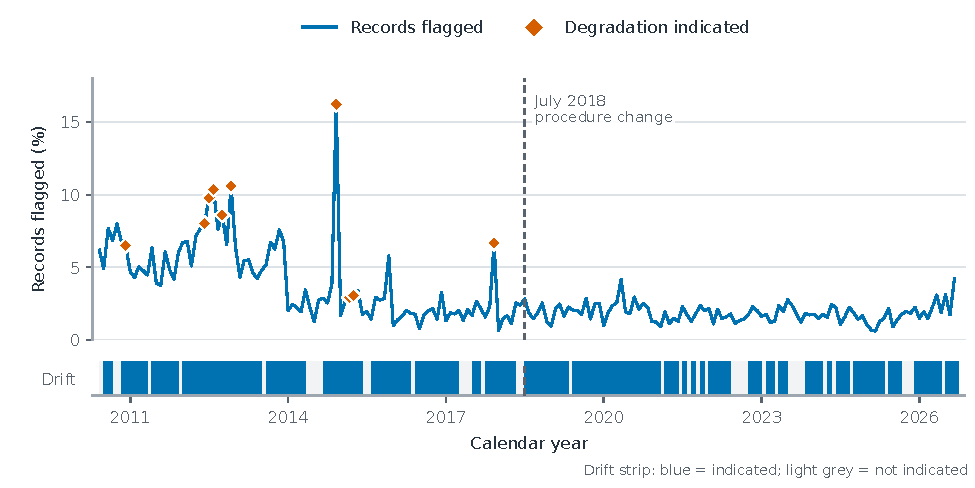
\includegraphics[width=\linewidth]{figures/chicago_temporal.pdf}
\caption{Chronological replay of raw Chicago food-inspection records using the rolling drift reference and all checks, over 196 evaluated months (June 2010--September 2026). The upper panel shows the percentage of flagged records; diamonds identify months labelled degradation, including drift with degradation. The lower strip shows months with a drift indication in blue and other months in light grey. The dashed line marks the documented procedure change on 1 July 2018. These are monitor outputs, not exhaustive ground-truth labels for all changes.}
\Description{A monthly line chart shows the flagged-record percentage from 2010 to 2026, with ten diamond markers at degradation indications. A lower monthly strip distinguishes drift indications from other months. A dashed vertical line marks the July 2018 inspection-procedure change. The flagged percentage is generally higher before 2015 and mostly lower afterward, while drift is indicated in many months.}
\label{fig:replay}
\end{figure}

The rolling-reference monitor labels most months as drift. Monthly batches average about 1,580 records, so comparatively small changes in category mixtures can exceed thresholds calibrated on five initial months. The minimum-effect-size variant reduces drift-only months from 143 to 74 while retaining the July 2018 transition. Against the original warm-up, 195 of 196 months are labelled drift. This demonstrates the operational importance of reference choice and effect size, rather than establishing that all such alarms identify meaningful change.

Some alarms can be assessed under the stated schema and domain policy without injected labels. Missing monitored values are errors under that policy. Risk and result values that remain inside their documented domains are admissible, so category-list alarms on those values are false alarms under domain membership; this does not establish the factual correctness of each inspection record. Facility Type has 3,276 alarms across 433 distinct values. Human adjudication remains outstanding for all of them. A provisional triage combines deterministic format-variant rules (40 values, 573 alarms) with model suggestions for the remaining values, assigning approximately 93\% of alarms to non-error, 3.5\% to error and 3.5\% to unclear. These are suggestions for review, not human-validated precision. Overlapping check-record alarms are not summed as distinct erroneous records.

\subsection{Sensitivity Analysis}
\label{sec:res:sens}

Five claims were re-checked while one setting at a time was changed and everything else stayed frozen (Table~\ref{tab:sens}). Five dials were prespecified before freezing: the error rate (1 to 20\%), outlier severity, the drift and degradation multiplier $z$ (2 to 4), the risk weights (each weight multiplied by 0, 0.5 or 2, and equal weights) and the risk thresholds. Three dials were added after freezing and are reported as post-hoc: the range multiplier $k$ (2.5 to 4), the history window (3 to 10 batches) and the drift budget $\alpha$ (0.01 to 0.20).

\begin{table}[t]
\caption{Sensitivity criterion counts on their assigned scenario subsets, ten test seeds per setting. H1a uses A/B, not contamination F1/F2. C1/C2 use paired interval criteria; C3--C5 are descriptive point comparisons, and C5 concerns sustained degradation C/D.}
\label{tab:sens}
\footnotesize
\begin{tabular}{@{}lrrr@{}}
\toprule
Claim & BTS & Chicago & Retail \\
\midrule
\inputtable{tables/sensitivity.tex}
\bottomrule
\end{tabular}
\end{table}

BTS and Chicago meet every listed criterion over the settings and scenario subsets assigned to it. This does not overturn their persistent-contamination failures, because the H1a sensitivity grid uses A/B rather than F1/F2. On Retail, the FPR-related and comparative macro-F1 criteria fail in all tested settings, including default settings; these failures are therefore stable within this sensitivity grid rather than dependent on one parameter choice. Two other verdicts vary: mild-outlier recall non-inferiority on Retail, whose difference is $+2.4$ pp with a lower bound of $-1.45$ pp, and usefulness of risk selection at moderate-risk threshold 0.10. One-at-a-time sensitivity describes these tested perturbations; it does not establish robustness to all joint parameter changes.

\subsection{Summary of Verdicts}

Table~\ref{tab:verdicts} collects the decisions without pooling unlike datasets. It distinguishes failure to meet a prespecified criterion, identical observed predictions, absence of detected superiority, ceiling-limited coverage and point-estimate scheduling usefulness. These distinctions are necessary to connect the evidence back to RQ1--RQ3 without extending the hypotheses after seeing the outcomes.

\begin{table}[t]
\caption{Summary of hypothesis verdicts on the confirmatory test run.}
\label{tab:verdicts}
\footnotesize
\begin{tabularx}{\linewidth}{@{}lXXX@{}}
\toprule
Hypothesis & BTS & Chicago & Retail \\
\midrule
H1a lower FPR, recall non-inferior & Supported in 6 of 9 scenarios; fails under mild errors without drift and under contamination & Supported in 9 of 9; margin 0.03 pp, from the category policy & Not supported (0 of 9); lower FPR not established, recall often higher \\
H1b four-class labelling & Supported; better than all comparators & Identical to gated fixed and EWMA on these runs & No detected advantage over gated fixed or EWMA \\
H2a validated LLM rules add coverage & Supported ($+0.48$) & Undecidable (ceiling at 1.00) & Supported ($+0.49$) \\
H2b guarded admission & Supported for per-value check; not for list or pattern constraints & Partly: one of four invalid values admitted by per-value check & Supported for per-value check \\
H3 risk-based selection useful & 4 of 6 cases (mean criterion) & 4 of 6 cases (mean criterion) & 3 of 6 cases (mean criterion) \\
\bottomrule
\end{tabularx}
\end{table}
